\documentclass[tikz,border=8pt]{standalone}

\usepackage[utf8]{inputenc}
\usepackage[T1]{fontenc}
\usepackage{lmodern}
\usepackage{xcolor}
\usetikzlibrary{arrows.meta,calc,positioning}
\renewcommand{\familydefault}{\sfdefault}

\definecolor{medPurple}{HTML}{9B456F}
\definecolor{medBlue}{HTML}{249DC4}
\definecolor{latentGray}{HTML}{5A5A5A}
\definecolor{lossYellow}{HTML}{F1D897}
\definecolor{taskGreen}{HTML}{6EB79B}
\definecolor{panelGray}{HTML}{CFCFCF}
\definecolor{jepaOrange}{HTML}{E8893A}
\definecolor{removeRed}{HTML}{B50000}
\definecolor{patchGray}{HTML}{B7B7B7}

\tikzset{
  font=\sffamily,
  arrow/.style={-{Latex[length=2.0mm,width=1.7mm]}, draw=black, line width=1.1pt},
  dotarrow/.style={-{Latex[length=2.0mm,width=1.7mm]}, draw=black!60, dotted, line width=1.25pt},
  backarrow/.style={-{Latex[length=2.0mm,width=1.6mm]}, draw=jepaOrange!90!black, dashed, line width=1.05pt},
  panel/.style={rounded corners=8pt, draw=panelGray, dashed, line width=1.35pt, fill=white},
  image/.style={rectangle, draw=black, line width=0.75pt, fill=black!18, minimum width=2.1cm, minimum height=1.25cm, align=center, inner xsep=5pt, inner ysep=4pt, font=\bfseries\small},
  model/.style={rectangle, rounded corners=2pt, draw=none, fill=medPurple, text=white, minimum width=1.75cm, minimum height=1.02cm, align=center, inner xsep=6pt, inner ysep=4pt, font=\bfseries\small},
  frozen/.style={rectangle, rounded corners=2pt, draw=none, fill=medBlue, text=white, minimum width=1.75cm, minimum height=1.02cm, align=center, inner xsep=6pt, inner ysep=4pt, font=\bfseries\small},
  latent/.style={rectangle, draw=none, fill=latentGray, text=white, minimum width=1.75cm, minimum height=0.84cm, align=center, inner xsep=6pt, inner ysep=4pt, font=\bfseries\small},
  predictor/.style={rectangle, rounded corners=2pt, draw=none, fill=jepaOrange, text=white, minimum width=2.3cm, minimum height=0.92cm, align=center, inner xsep=7pt, inner ysep=4pt, font=\bfseries\small},
  loss/.style={rectangle, draw=none, fill=lossYellow, minimum width=3.7cm, minimum height=0.45cm, align=center, inner xsep=6pt, inner ysep=3pt, font=\bfseries\scriptsize},
  task/.style={rectangle, rounded corners=2pt, draw=none, fill=taskGreen, text=white, minimum width=3.25cm, minimum height=0.92cm, align=center, inner xsep=8pt, inner ysep=4pt, font=\bfseries\small},
  detail/.style={rectangle, rounded corners=2pt, draw=black!35, line width=0.5pt, fill=white, minimum width=2.35cm, minimum height=0.82cm, align=center, inner xsep=6pt, inner ysep=4pt, font=\bfseries\small},
  title/.style={font=\sffamily\bfseries\Large, align=center},
  panelLetter/.style={font=\sffamily\bfseries\LARGE},
  smallLabel/.style={font=\sffamily\scriptsize},
  flowLabel/.style={font=\sffamily\scriptsize, inner sep=1.4pt},
  redNote/.style={font=\sffamily\bfseries\small, text=removeRed}
}

\newcommand{\patchGrid}[3]{%
  \coordinate (#1west) at ($(#2,#3)+(-0.9,0)$);
  \coordinate (#1east) at ($(#2,#3)+(0.9,0)$);
  \coordinate (#1north) at ($(#2,#3)+(0,0.9)$);
  \coordinate (#1south) at ($(#2,#3)+(0,-0.9)$);
  \fill[patchGray] ($(#2,#3)+(-0.9,-0.9)$) rectangle ($(#2,#3)+(0.9,0.9)$);
  \foreach \x in {-0.9,-0.45,0,0.45,0.9} {
    \draw[white, line width=0.35pt] ($(#2,#3)+(\x,-0.9)$) -- ($(#2,#3)+(\x,0.9)$);
    \draw[white, line width=0.35pt] ($(#2,#3)+(-0.9,\x)$) -- ($(#2,#3)+(0.9,\x)$);
  }
  \fill[white] ($(#2,#3)+(-0.45,0.45)$) rectangle ($(#2,#3)+(0,0.9)$);
  \fill[white] ($(#2,#3)+(0.45,0)$) rectangle ($(#2,#3)+(0.9,0.45)$);
  \fill[white] ($(#2,#3)+(0,-0.45)$) rectangle ($(#2,#3)+(0.45,0)$);
  \fill[white] ($(#2,#3)+(-0.9,-0.9)$) rectangle ($(#2,#3)+(-0.45,-0.45)$);
  \draw[black, line width=0.75pt] ($(#2,#3)+(-0.9,-0.9)$) rectangle ($(#2,#3)+(0.9,0.9)$);
}

\newcommand{\freezeMark}[1]{%
  \begin{scope}[shift={($(#1.north east)+(-0.18,-0.18)$)}, scale=0.12]
    \draw[white, line width=0.75pt] (-1,0) -- (1,0);
    \draw[white, line width=0.75pt] (0,-1) -- (0,1);
    \draw[white, line width=0.75pt] (-0.72,-0.72) -- (0.72,0.72);
    \draw[white, line width=0.75pt] (-0.72,0.72) -- (0.72,-0.72);
  \end{scope}
}

\begin{document}
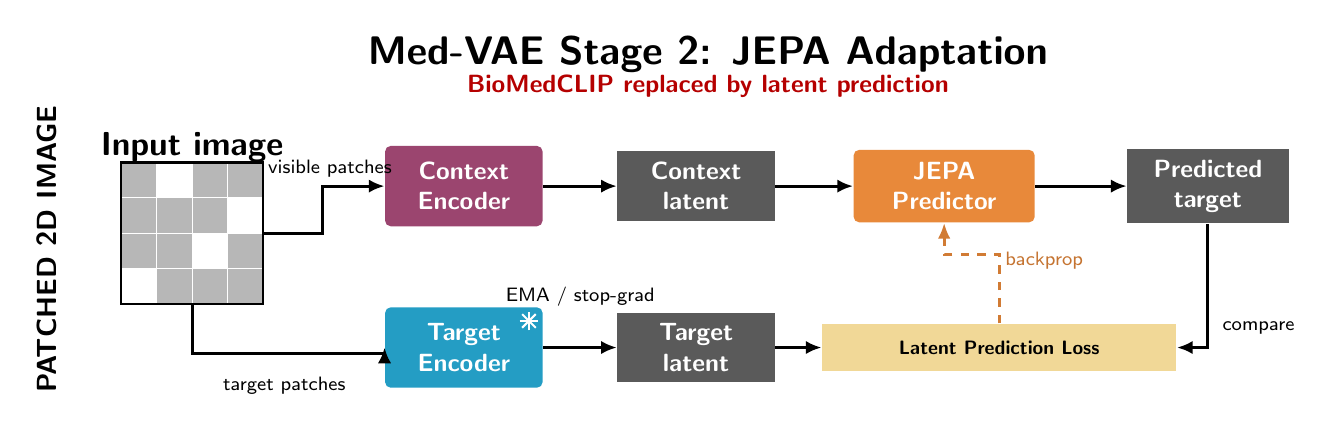
\begin{tikzpicture}[x=1cm,y=1cm]

% --------------------------------------------------------------------------
% Panel b — Med-VAE Stage 2: JEPA Adaptation
% --------------------------------------------------------------------------
\node[title] at (9.3,4.92) {Med-VAE Stage 2: JEPA Adaptation};
\node[redNote] at (9.3,4.52) {BioMedCLIP replaced by latent prediction};

\node[font=\sffamily\bfseries\normalsize, rotate=90] at (0.9,2.45) {PATCHED 2D IMAGE};
\node[font=\sffamily\bfseries\large] at (2.75,3.75) {Input image};
\patchGrid{patches}{2.75}{2.65}

\node[model, minimum width=2.0cm] (bCtx) at (6.2,3.25) {Context\\Encoder};
\node[latent, minimum width=2.0cm] (bCtxLat) at (9.15,3.25) {Context\\latent};
\node[predictor] (bPred) at (12.3,3.25) {JEPA\\Predictor};
\node[latent, minimum width=2.05cm] (bPredLat) at (15.65,3.25) {Predicted\\target};

\node[frozen, minimum width=2.0cm] (bTgt) at (6.2,1.2) {Target\\Encoder};
\freezeMark{bTgt}
\node[latent, minimum width=2.0cm] (bTgtLat) at (9.15,1.2) {Target\\latent};
\node[loss, minimum width=4.5cm, minimum height=0.6cm] (bLoss) at (13.0,1.2) {Latent Prediction Loss};

\draw[arrow] (patcheseast) -- ++(0.75,0) |- (bCtx.west);
\node[flowLabel, anchor=south] at (4.5,3.3) {visible patches};
\draw[arrow] (patchessouth) -- ++(0,-0.62) -| (bTgt.west);
\node[flowLabel, anchor=north] at (3.92,0.88) {target patches};
\draw[arrow] (bCtx.east) -- (bCtxLat.west);
\draw[arrow] (bCtxLat.east) -- (bPred.west);
\draw[arrow] (bPred.east) -- (bPredLat.west);
\draw[arrow] (bTgt.east) -- (bTgtLat.west);
\node[flowLabel, anchor=south] at (7.68,1.67) {EMA / stop-grad};
\draw[arrow] (bTgtLat.east) -- (bLoss.west);
\coordinate (bCompareElbow) at (15.65,1.2);
\draw[arrow] (bPredLat.south) -- (bCompareElbow) -- (bLoss.east);
\node[flowLabel, anchor=west] at (15.78,1.45) {compare};
\draw[backarrow] (bLoss.north) -- ++(0,0.88) -| (bPred.south);
\node[flowLabel, text=jepaOrange!85!black, anchor=west] at (13.02,2.3) {backprop};

\end{tikzpicture}
\end{document}
